% Relatório do laboratório 5 de servo
% Felipe Bandeira da Silva
% 27/09/2013

%\documentclass[a4paper, 10pt]{article}
\documentclass[paper=a4, fontsize=11pt]{article}


\usepackage[brazil]{babel}
\usepackage[utf8]{inputenc}
\usepackage{listings}
\usepackage{color}
\usepackage{amsthm}
\usepackage{graphicx}

\usepackage{schemabloc}
\usetikzlibrary{circuits}

\usepackage{tabularx,ragged2e,booktabs,caption}

\setlength{\parindent}{0pt}
\setlength{\parskip}{18pt}

\title{\textsc{Laboratório Transformadores\\Transformadores em Paralelo}}
\author{Felipe Bandeira da Silva\\1020942-X}
%\date{}

\begin{document}


\maketitle

%\newpage

%\begin{abstract}
\textit{Este laboratório tem como objetivo: Identificar e ligar uma transformação delta aberto. Identificar e ligar uma transfomação Triângulo-Triângulo, Triângulo-Estrela. Identificar e ligar conexões zero graus e cento e oitenta graus.}
%\end{abstract}

\newpage

\tableofcontents

\newpage

\listoffigures


%%%%%%%%%%%%%%%%%%%%%%%%%%%%%%%%%%%%%%%%%%%%%%%%%%%%%%%%%%%%%%%%%%%%%%%%%%%%%%%%
% fundamentação teórica
\newpage
\section{Fundamentação Teórica}

Para transformar-se a tensão de uma fonte trifásica, se requer ou uma bancada de
transformadores monofásicos, como mostra a Fig. 1, ou, alternativamente um único
transformador trifásico com seis enrolamentos num núcleo comum de ferro. Vale 
salientar que os transformadores são idênticos ou seja, tem a mesma potência, mesma
relação de alta para baixa tensão.

\begin{figure}[!ht]
    \centering
    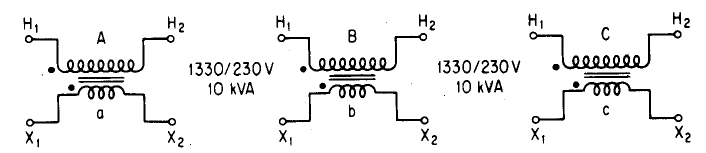
\includegraphics[scale=.6]{mono3}
    \caption{Transformação trifásica com transformadores monofásicos}
\end{figure}

Nota-se também que os transformadores têm as fases indicadas e apropriadamente marcadas,
de maneira que o subíndice impar mostra polaridade instantânea positiva. 
O uso de transformadores monofásicos em conexões trifásicas obedecem critérios que 
vão desde a continuidade de serviço, a confiabilidade do sistema, a limitação
do tamanho de fabricação de um único trifásico, qualidade de energia.

\section{Identificação de cada transformador}

A primeira parte da experiência é referente a identificação do transformador monofásico
utilizado.

\subsection{Tensão de cada transformador}
\renewcommand{\arraystretch}{1.5}
\begin{center}
    \begin{tabular}{c||c}
        1.2 | 3.4 & 208 [V] \\
        5.6 | 7.8 & 208 [V] \\
        9.10 | 11.12 & 208 [V] \\
    \end{tabular}
    \captionof{table}{}
\end{center}

\subsection{Polaridade dos terminais}

Positivo do transformador 1: pino 1\\
Positivo do transformador 2: pino 5\\
Positivo do transformador 3: pino 9\\

\section{Ligação em Triângulo}

Para essa parte é necessário alimentar o módulo com tensão trifásica na sequencia 
positiva. Foram colocados voltímetros na entrada trifásica e na saída trifásica e 
amperímetros apenas na entrada. A tensão de alimentação fase-fase foi elevada 
gradativamente até aproximadamente 208 Volts. As seguintes tensões foram mensuradas
no secundário,


\begin{center}
    \begin{tabular}{c||c}
        $V_1$ & 210 [V] \\
        $V_2$ & 211 [V] \\
        $V_3$ & 209 [V] \\
    \end{tabular}
    \captionof{table}{}
\end{center}

Com dois transformadores monofásicos podemos criar um sistema trifásico com tensões
defasadas de 120º. Neste caso haverá uma redução de potência de cada transformador
de 33 $\%$

\section{Ligação Triângulo-Triângulo}
\begin{figure}[!ht]
    \centering
    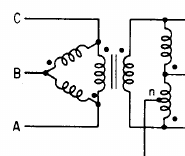
\includegraphics[scale=.8]{delta}
    \caption{Ligação Estrela-Estrela}
\end{figure}
Para tanto a seguintes tensões foram medidas,

\begin{center}
    \begin{tabular}{c||c}
        $V_1$ & 225 [V] \\
        $V_2$ & 225 [V] \\
        $V_3$ & 220 [V] \\
    \end{tabular}
    \captionof{table}{}
\end{center}

Comentário: Tensões de fase-fase da saída do secundário, sequencia positiva.

\begin{center}
    \begin{tabular}{c||c}
        $V_1$ & 225 [V] \\
        $V_2$ & 225 [V] \\
        $V_3$ & 220 [V] \\
    \end{tabular}
    \captionof{table}{}
\end{center}

Comentário: Tensões de fase-fase da saída do secundário, sequencia negativa.

\section{Ligação Estrela-Estrela}

As seguintes medidas foram feitas, tomando como ponto de referência as tensões de 
fase-neutro.

\begin{figure}[!ht]
    \centering
    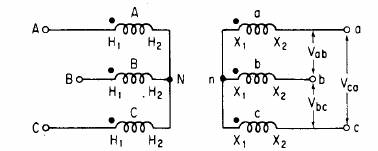
\includegraphics[scale=.8]{estrela}
    \caption{Ligação Estrela-Estrela}
\end{figure}

\begin{center}
    \begin{tabular}{c||c}
        $V_1$ & 130.0 [V] \\
        $V_2$ & 129.0 [V] \\
        $V_3$ & 129.7 [V] \\
    \end{tabular}
    \captionof{table}{}
\end{center}

\section{Conclusão}
Conclui-se com esta prática a importância das devidas ligações de uma transformador
é se os devidos cuidados não forem considerados é possível danificar o transformador
ou enviar a sequencia errónea para a carga. Importante salientar a devida atenção à
polaridade instantânea não pode ser desprezada, quer ao se ligarem secundários em 
paralelo, quer ao se acertarem as tensões secundárias e sua relação de fase.

\end{document}
